\section[Algorithme Bayésien Naïf]{Algorithme Bayésien Naïf}

\subsection[Cas d'utilisation]{Cas d'utilisation}

\begin{frame}{Présentation du cas d'utilisation}
	Nous allons utiliser comme support des données textuelles: des critiques de films, afin de réaliser une \textbf{analyse de sentiment}.
	\begin{itemize}
		\item Nous allons utiliser une base de données de critiques de films postées par les utilisateurs du site anglophone \href{https://m.imdb.com/}{IMDb}: \url{https://www.kaggle.com/datasets/yasserh/imdb-movie-ratings-sentiment-analysis}
		\item Ces critiques sont soit positives, soit négatives.
		\item Nous allons donc construire un classifieur binaire pour associer une critique à une opinion (positive ou négative).
	\end{itemize}
	Un algorithme Bayésien Naïf est un très bon candidat pour ce genre de problème ! 
\end{frame}

\begin{frame}{Challenge}
	Il y a donc un double challenge !
	\begin{itemize}
		\item Comment traite-t-on des données textuelles avec un algorithme d'apprentissage automatique ?
		\item Comment est-ce qu'on peut utiliser le théorème de Bayes avec ces données ?
	\end{itemize}
\end{frame}

\begin{frame}{Données de travail}
	Supposons que nous avons collecté des exemples de critiques positives et négatives. Nous avons \textbf{compté} combien de fois certains mots apparaissent dans les critiques:
	\begin{columns}
		\begin{column}{0.5\textwidth}
			\begin{figure}
				\centering
				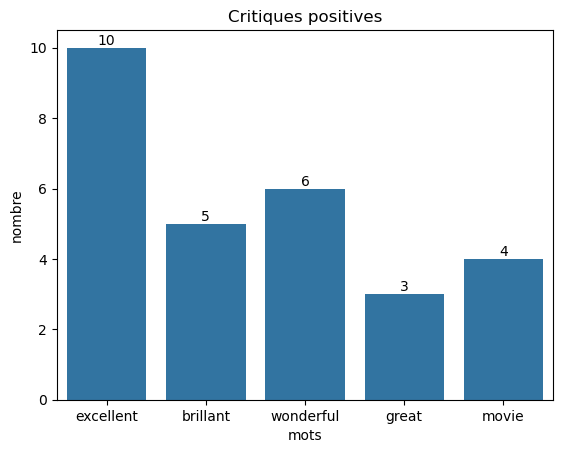
\includegraphics[width=1.0\linewidth]{Images/critiques_positives}
				\label{fig:critiques_positives}
			\end{figure}
		\end{column}
		\begin{column}{0.5\textwidth}
			\begin{figure}
				\centering
				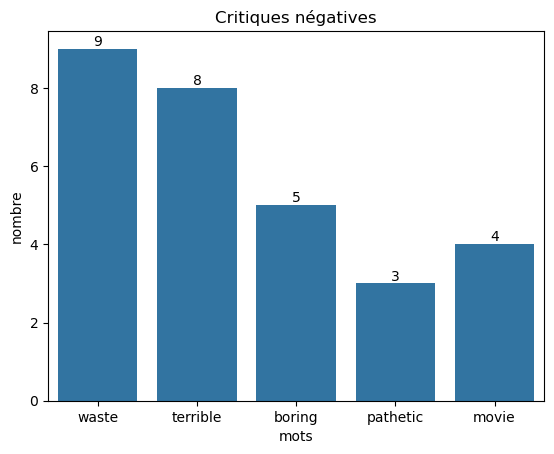
\includegraphics[width=1.0\linewidth]{Images/critiques_negatives}
				\label{fig:critiques_negatives}
			\end{figure}
		\end{column}		
	\end{columns}	
\end{frame}

\begin{frame}{Données de travail - Probabilités}
	Nous pouvons facilement en dériver des \textbf{probabilités conditionnelles}. Elles sont conditionnelles dans le sens où on traite séparément les critiques positives et les critiques négatives:
	\begin{columns}
		\begin{column}{0.5\textwidth}
			\begin{figure}
				\centering
				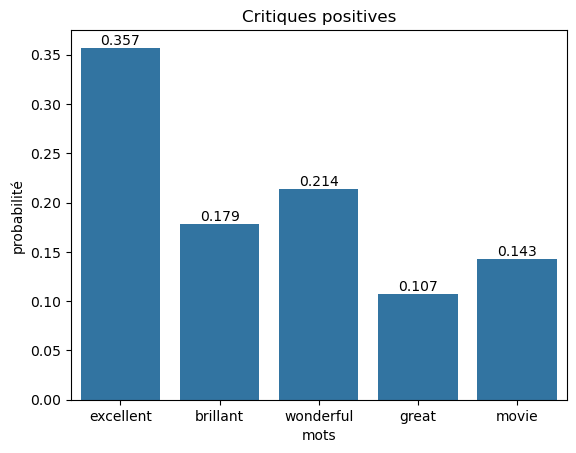
\includegraphics[width=1.0\linewidth]{Images/critiques_positives_probab}
				\label{fig:critiques_positives_probab}
			\end{figure}
		\end{column}
		\begin{column}{0.5\textwidth}
			\begin{figure}
				\centering
				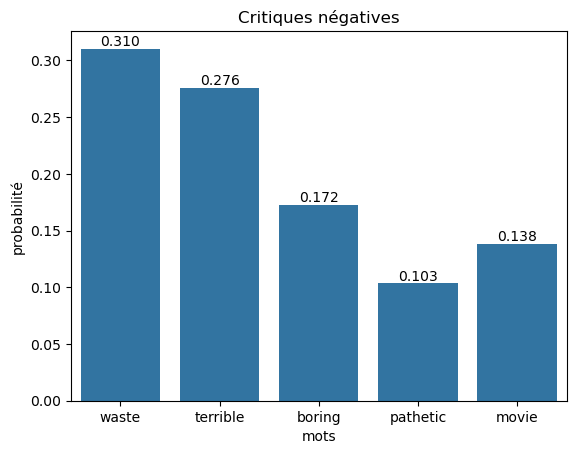
\includegraphics[width=1.0\linewidth]{Images/critiques_negatives_probab}
				\label{fig:critiques_negatives_probab}
			\end{figure}
		\end{column}		
	\end{columns}	
\end{frame}

\begin{frame}{Première tentative de calcul}
	\begin{itemize}
		\item Nous appellerons $C$ la variable aléatoire discrète $C \in \{0, 1\}$ qui désigne le sentiment associée à une critique.
		\pause
		\item  $C$ vaut 1 si la critique est positive et 0 sinon.	Supposons que la probabilité a priori est équilibrée: $P(C = 0) = 0.5$ et $P(C = 1) = 0.5$.
		\pause
		\item La critique qui nous intéresse est la suivante: \textit{brilliant}. Comment calculer une probabilité a posteriori ?
	\end{itemize}
	\pause
	Une façon de faire serait de calculer le facteur de Bayes:
	\begin{equation}
		\text{BF}_{10}(\text{"brilliant"}) = \frac{P(\text{"brilliant"} \mid C = 1)}{P(\text{"brilliant"} \mid C = 0)}
		\nonumber
	\end{equation}
	Mais il y a un petit problème: $P(\text{"brilliant"} \mid C = 0) = 0$. On aurait donc un facteur de Bayes infini !
\end{frame}

\begin{frame}{Données de travail - Lissage de Laplace}
	Nous allons transformer les données en utilisant un \textbf{lissage de Laplace}. Au lieu de calculer les probabilités conditionnelles comme ceci:
	\begin{equation}
		P(\text{mot} \mid C = K) = \frac{\text{nombre d'occurrences de mot quand } C = K}{\text{nombre total d'occurrences quand }C = K}
		\nonumber
	\end{equation}
	\pause
	On va les calculer comme ceci:
	\begin{equation}
		\begin{split}
			&P(\text{mot} \mid C = K) = \\
			&\frac{\text{nombre d'occurrences de mot quand } C = K + \color{red}1}{\text{nombre total occurrences quand } C = K + \color{red} \text{nombre total de mots différents}}
		\end{split}
		\nonumber
	\end{equation}
	\pause
	Cela consiste simplement à ajouter chaque mot une fois à l'ensemble des classes (critique positive et critique négative).
\end{frame}

\begin{frame}{Données de travail - Lissage de Laplace}
	Une fois le lissage de Laplace appliqué, nous avons donc:
	\begin{columns}
		\begin{column}{0.5\textwidth}
			\begin{figure}
				\centering
				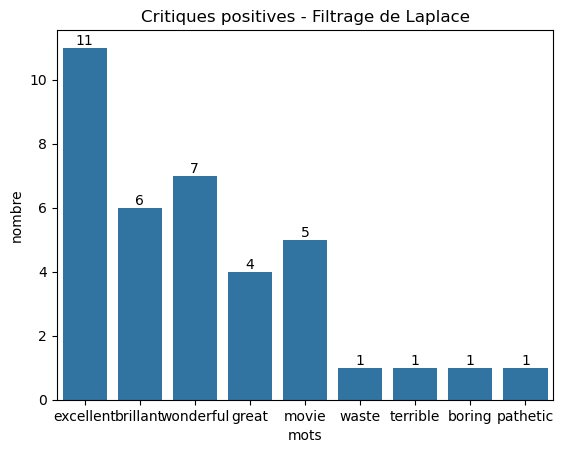
\includegraphics[width=1.0\linewidth]{Images/critiques_positives_laplace}
				\label{fig:critiques_positives_laplace}
			\end{figure}
		\end{column}
		\begin{column}{0.5\textwidth}
			\begin{figure}
				\centering
				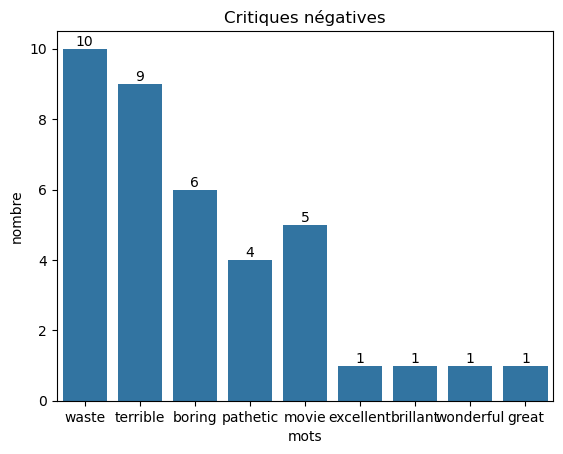
\includegraphics[width=1.0\linewidth]{Images/critiques_negatives_laplace}
				\label{fig:critiques_negatives_laplace}
			\end{figure}
		\end{column}		
	\end{columns}	
\end{frame}

\begin{frame}{Données de travail - Probabilités avec lissage de Laplace}
	Et les nouvelles probabilités conditionnelles:
	\begin{columns}
		\begin{column}{0.5\textwidth}
			\begin{figure}
				\centering
				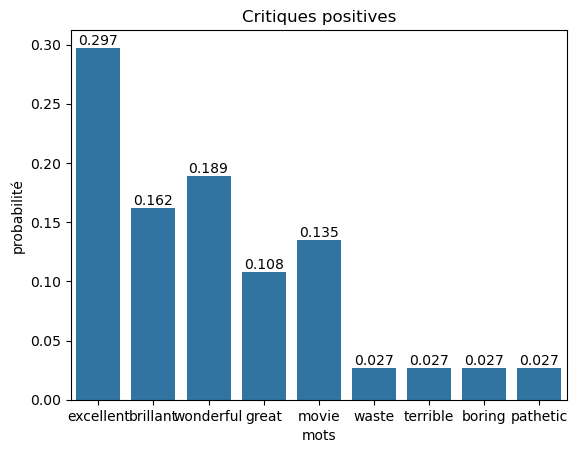
\includegraphics[width=1.0\linewidth]{Images/critiques_positives_probab_laplace}
				\label{fig:critiques_positives_probab_laplace}
			\end{figure}
		\end{column}
		\begin{column}{0.5\textwidth}
			\begin{figure}
				\centering
				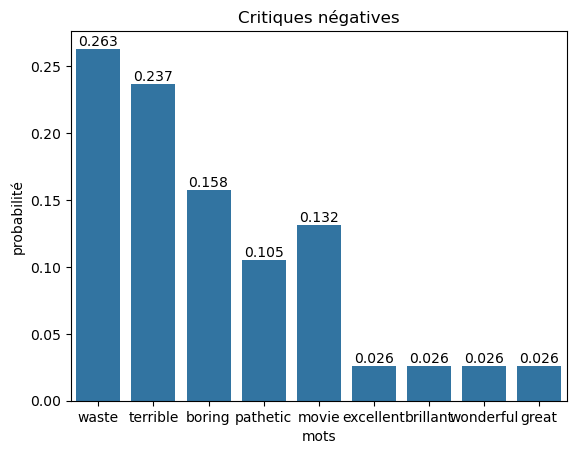
\includegraphics[width=1.0\linewidth]{Images/critiques_negatives_probab_laplace}
				\label{fig:critiques_negatives_probab_laplace}
			\end{figure}
		\end{column}		
	\end{columns}	
\end{frame}

\subsection[Calculs des probabilités]{Calculs des probabilités}

\begin{frame}{Premier calcul}
	\begin{itemize}
		\item  Supposons que la probabilité a priori est équilibrée: $P(C = 0) = 0.5$ et $P(C = 1) = 0.5$.
		\item La critique qui nous intéresse est la suivante: \textit{brilliant}. Comment calculer une probabilité a posteriori ?
	\end{itemize}
	\pause
	Une façon de faire serait de calculer le facteur de Bayes:
	\begin{equation}
		\begin{aligned}
			\text{BF}_{10}(\text{"brilliant"}) 
			&= \frac{P(\text{"brilliant"} \mid C = 1)}{P(\text{"brilliant"} \mid C = 0)} \\
			&= \frac{0.162}{0.026} \approx 6.23
		\end{aligned}
		\nonumber
	\end{equation}
	\pause
	La cote initiale étant de $1:1$, la cote finale devient $6.23:1$. Ce qui fait une probabilité a posteriori de 0.862.
\end{frame}

\begin{frame}{Premier calcul - Alternative}
	Une alternative consiste à calculer les 2 quantités suivantes qui correspondent aux numérateurs dans le théorème de Bayes:
	\begin{equation}
		\begin{cases}
			P(\text{"brilliant"} \mid C = 1) P(C=1) \\
			P(\text{"brilliant"} \mid C = 0) P(C=0)
		\end{cases}
		\nonumber
	\end{equation}
	\pause
	On ne s'embarrasse pas du dénominateur $P(\text{"brilliant"})$, vu que la somme des probabilités a posteriori doit être égale à 1:
	\begin{equation}
		\begin{cases}
			P(C = 1 \mid \text{"brilliant"}) \propto P(\text{"brilliant"} \mid C = 1) P(C=1) \\
			P(C = 0 \mid \text{"brilliant"}) \propto P(\text{"brilliant"} \mid C = 0) P(C=0)
		\end{cases}
		\nonumber
	\end{equation}
	C'est ce qui est implémenté dans l'algorithme Bayésien Naïf.
\end{frame}

\begin{frame}{Premier calcul - Alternative}
	On peut vérifier que cela mène au même résultat:
	\begin{equation}
		\begin{cases}
			P(\text{"brilliant"} \mid C = 1) P(C=1) = 0.162 \times 0.5 = 0.081 \\
			P(\text{"brilliant"} \mid C = 0) P(C=0) = 0.026 \times 0.5 = 0.013
		\end{cases}
		\nonumber
	\end{equation}	
	En normalisant, on obtient:
	\begin{equation}
		\begin{cases}
			P(C = 1 \mid \text{"brilliant"}) = 0.081 / (0.081 + 0.013) =  0.862 \\
			P(C = 0 \mid \text{"brilliant"}) = 0.013 / (0.081 + 0.013) =  0.138
		\end{cases}
		\nonumber
	\end{equation}
	On obtient, bien entendu, le même résultat. C'est la méthode implémentée dans un algorithme Bayésien Naïf.
\end{frame}

\subsection[Hypothèses de l'algorithme Bayésien Naïf]{Hypothèses de l'algorithme Bayésien Naïf}

\begin{frame}{Une critique plus élaborée}
	Supposons maintenant que la critique est \textit{boring movie, waste of time}:
	\begin{itemize}
		\item Les mots \text{of} et \text{time} ne font pas partie du \textbf{vocabulaire} que nous avons considéré.
		\pause
		\item Nous allons donc ignorer ces termes.
		\pause
		\item La ponctuation n'est pas non plus gérée. On va aussi s'en séparer. La critique est donc \textit{boring movie waste}.
		\pause
		\item Nous cherchons donc à calculer: $P(C = 1 \mid \text{"boring movie waste"})$ qui nécessite de connaitre la vraisemblance $P(\text{"boring movie waste"} \mid C = 1)$.
		\pause
		\item Mais nous ne connaissons pas la probabilité jointe de ces mots ! Ils sont forcément liés. Une phrase n'est pas juste un empilement de mots pris au hasard.
	\end{itemize}
	\pause
	C'est là que la nature \textbf{naïve} de l'algorithme intervient. Pour simplifier, on va considérer que les mots au sein d'une même phrase sont indépendants. C'est \textbf{faux} mais cela simplifie grandement les calculs !
\end{frame}

\begin{frame}{Nature naïve de l'algorithme}
	\begin{itemize}
		\item C'est là que la nature \textbf{naïve} de l'algorithme intervient.
		\pause
		\item Pour simplifier, on va considérer que les mots au sein d'une même phrase sont indépendants.
		\pause
		\item C'est \textbf{simpliste} mais bien pratique pour faire les calculs !
	\end{itemize}
	\pause
	\vspace{0.5cm}
	C'est comme dans tous les exemples traités jusqu'à maintenant. On a pris pour hypothèse que les tests Covid 19 étaient indépendants. De même que les critiques de films. Et ici on considère les mots au sein d'une même phrase comme indépendants !
\end{frame}

\begin{frame}{Nature multinomiale de l'algorithme}
	\begin{itemize}
		\item Rappel, notre critique simplifiée est: \textit{boring movie waste}.
		\pause
		\item On considère chaque mot comme indépendant. Donc Il s'agit de faire 3 mises à jour avec le théorème de Bayes, ou multiplier 3 facteurs de Bayes.
		\pause
		\item La différence avec nos exemples précédents c'est que chaque mot apporte une conviction \textbf{différente}: les facteurs de Bayes sont différents pour chaque mots, c'est la nouveauté.
		\pause
		\item C'est pour cette raison que cet algorithme est appelé algorithme Bayésien Naïf \textbf{multinomial}. 
		\pause
		\item Multinomial fait allusion à la nature de la distribution de probabilité. Nos exemples précédents utilisaient une distribution de Bernoulli !
		\pause
		\item Notre algorithme utilise 2 distributions multinomiales, une pour les critiques négatives et une pour les critiques positives. Les tracés graphiques avec les probabilités vus précédemment sont en fait les tracés des fonctions de masse de ces distributions. !
	\end{itemize}
\end{frame}

\begin{frame}{Une critique plus élaborée - Calcul}
	\begin{equation}
		\resizebox{1.0\textwidth}{!}{%
			$\begin{cases}
				P(C = 0 \mid \text{"boring movie waste"}) \propto P(\text{"boring movie waste"} \mid C = 0) P(C=0) \\
				P(C = 1 \mid \text{"boring movie waste"}) \propto P(\text{"boring movie waste"} \mid C = 1) P(C=1)
			\end{cases}$
		}
		\nonumber
	\end{equation}
	\pause
	Avec l'hypothèse d'indépendance naïve on peut écrire:
	\begin{equation}
		\begin{aligned}
			&P(\text{"boring movie waste"} \mid C = 0) P(C=0) \\
			&= P(\text{"boring"} \mid C = 0) P(\text{"movie"} \mid C = 0) P(\text{"waste"} \mid C = 0) P(C=0) \\
			&= 0.158 \times 0.132 \times 0.263 \times 0.5 \\
			&\approx 0.00274 
		\end{aligned}
		\nonumber
	\end{equation}
	\pause
	Similairement:
	\begin{equation}
		\begin{aligned}
			&P(\text{"boring movie waste"} \mid C = 1) P(C=1) \\
			&= P(\text{"boring"} \mid C = 1) P(\text{"movie"} \mid C = 1) P(\text{"waste"} \mid C = 1) P(C=1) \\
			&= 0.027 \times 0.135 \times 0.027 \times 0.5 \\
			&\approx 0.00005
		\end{aligned}
		\nonumber
	\end{equation}
\end{frame}

\begin{frame}{Une critique plus élaborée - Calcul}
	Après normalisation, on obtient:
	\begin{equation}
		\begin{cases}
			P(C = 0 \mid \text{"boring movie waste"}) \approx 0.982 \\
			P(C = 1 \mid \text{"boring movie waste"}) \approx 0.018
		\end{cases}
		\nonumber
	\end{equation}
	\pause
	Les probabilités qui se multiplient donnent très vite des nombres très petits. Les algorithmes calculent les \textbf{logarithmes} des probabilités. Grâce à l'hypothèse d'indépendance, le logarithme du produit des probabilités devient la somme des logarithmes des probabilités.
\end{frame}

\begin{frame}{Une critique plus élaborée - Facteurs de Bayes}
	On pourrait calculer les facteurs de Bayes pour chaque mot:
	\begin{equation}
		\begin{cases}
			\text{BF}_{10}(\text{"boring"}) = P(\text{"boring"} \mid C = 1) / P(\text{"boring"} \mid C = 0) \approx 0.171 \\
			\text{BF}_{10}(\text{"movie"}) = P(\text{"movie"} \mid C = 1) / P(\text{"movie"} \mid C = 0) \approx 1.023 \\
			\text{BF}_{10}(\text{"waste"}) = P(\text{"waste"} \mid C = 1) / P(\text{"waste"} \mid C = 0) \approx 0.103
		\end{cases}
		\nonumber
	\end{equation}
	\pause
	\begin{itemize}
		\item Le mot \textit{movie} aura très peu d'influence sur le résultat car son facteur de Bayes est très proche de 1.
		\item Le mot \textit{waste} est celui qui apporte la plus grande conviction que la critique est négative.
		\item On peut très facilement dériver les facteurs de Bayes en divisant les 2 fonctions de masse des distributions multinomiales.
	\end{itemize}
\end{frame}

\subsection[Formulation de l'algorithme Bayésien Naïf]{Formulation de l'algorithme Bayésien Naïf}

\begin{frame}{Hypothèse d'indépendance conditionnelle}
	Soient $x \in \R^d$ une caractéristique d'entrée et une variable aléatoire discrète $C \in \{0, 1\}$.
	\vspace{0.3cm}
	\begin{block}{Hypothèse d'indépendance conditionnelle (Naïve)}
		On suppose qu'il y a une indépendance conditionnelle dans les éléments de $x$:
		\begin{equation}
			P(x_1, x_2, \cdots, x_d \mid C = k) = \prod_{i=1}^{d} P(x_i \mid C = k) \quad k \in \{0, 1\}
			\nonumber
		\end{equation}
	\end{block}
\end{frame}

\begin{frame}{Maximum a posteriori}
	\begin{block}{Règle de décision (Maximum A Posteriori)}
		On cherche la classe qui maximise le produit de la probabilité a priori et de la vraisemblance:
		\begin{equation}
			\hat{y} = \argmax{k \in \{0, 1\}} \left( P(C = k) \prod_{i=1}^{d} P(x_i \mid C = k) \right)
			\nonumber
		\end{equation}
	\end{block}
	\pause
	Note: L'hypothèse naïve \textit{biaise} la probabilité a posteriori, mais comme nous ne recherchons que le maximum a posteriori, l'impact de cette hypothèse simpliste est limité sur les cas d'application.
\end{frame}

\begin{frame}{Passage au Logarithme}
	Pour éviter les erreurs de précision numérique et transformer les produits en sommes:
	\begin{block}{Règle de décision (Maximum A Posteriori)}
		On cherche la classe qui maximise le logarithme du produit de la probabilité a priori et de la vraisemblance:
		\begin{equation}
			\hat{y} = \argmax{k \in \{0, 1\}} \left( \ln P(C = k) + \sum_{i=1}^{d} \ln P(x_i \mid C = k) \right)
			\nonumber
		\end{equation}
	\end{block}
	\pause
	\begin{itemize}
		\item C'est l'implémentation de  \href{https://scikit-learn.org/stable/modules/generated/sklearn.naive_bayes.MultinomialNB.html}{\texttt{sklearn.naive\_bayes.MultinomialNB}}.
	\end{itemize}
\end{frame}

\begin{frame}{Calcul des probabilités avec la fonction softmax}
	Une fois les logarithmes $\ln P(C = k \mid x_1, \cdots, x_d)$ calculés, on peut calculer les probabilités avec une fonction \textbf{softmax}:
	\begin{equation}
		\resizebox{1.0\textwidth}{!}{%
			$P(C = 1 \mid x_1, \cdots, x_d) = \frac{\exp{\left(\ln P(C = 1  \mid x_1, \cdots, x_d)\right)}}{\exp{\left(\ln P(C = 1  \mid x_1, \cdots, x_d)\right)} + \exp{\left(\ln P(C = 0  \mid x_1, \cdots, x_d)\right)}}$
		}
		\nonumber
	\end{equation}
\end{frame}

\subsection[Combinaison d'algorithmes]{Combinaison d'algorithmes}

\begin{frame}{Cas d'étude}
	\begin{itemize}
		\item Sur le campus de l'université de Toulouse, à partir d'un échantillon d'étudiants et d'étudiantes on collecte la taille ainsi que l'UFR (Unité de Formation et de Recherche) comme Faculté de Santé, Lettres, Arts, Faculté des Sciences et de l'ingénierie.
		\pause
		\item On dispose de statistiques globales qui nous permettent de connaitre la répartition des étudiants (40\%) et des étudiantes (60\%). C'est notre probabilité a priori.
		\pause
		\item Nous pouvons établir deux distributions Gaussiennes pour la taille des étudiants et des étudiantes et utiliser ces distributions dans un algorithme Bayésien Naïf Gaussien.
		\pause
		\item Nous pouvons établir deux distributions multinomiales pour les UFR des étudiants et des étudiantes et utiliser ces distributions dans un algorithme Bayésien Naïf multinomial.
	\end{itemize}
\end{frame}

\begin{frame}{Cas d'étude - Calcul}
	\begin{itemize}
		\item Supposons que nous ayons un étudiant (ou une étudiante), dont nous connaissons la taille (172 cm) et l'UFR (Lettres). Quelle est la probabilité que ce soit une étudiante ?
		\pause
		\item On pourrait calculer les vraisemblances $\ln P(\text{Lettres} \mid \text{\'Etudiante})$ et $\ln P(\text{Lettres} \mid \text{\'Etudiant})$ en utilisant les distributions multinomiales. En fait, il s'agit de lire les fonctions de masse !
		\pause
		\item On pourrait calculer les vraisemblances $\ln P(\text{172 cm} \mid \text{\'Etudiante})$ et $\ln P(\text{172 cm} \mid \text{\'Etudiant})$ en utilisant les distributions Gaussiennes.
		\pause
		\item On ajoute ensuite ces vraisemblances à leur probabilité a priori: $\ln P(\text{Lettres} \mid \text{\'Etudiante}) + \ln P(\text{172 cm} \mid \text{\'Etudiante}) + \ln P(\text{\'Etudiante})$
		\pause
		\item Puis $\ln P(\text{Lettres} \mid \text{\'Etudiant}) + \ln P(\text{172 cm} \mid \text{\'Etudiant}) + \ln P(\text{\'Etudiant})$. 
		\pause
		\item On passe par la fonction softmax, et voilà !
	\end{itemize}
\end{frame}

\begin{frame}{Cas d'étude - Précisions pour l'algorithme Bayésien Naïf Gaussien}
	Pour une variable continue (taille), on ne compte plus des occurrences. On utilise la \textbf{loi normale}:
	\begin{equation}
		P(x \mid C=k) = \frac{1}{\sqrt{2\pi\sigma_k^2}} \exp\left(-\frac{(x-\mu_k)^2}{2\sigma_k^2}\right)
		\nonumber
	\end{equation}
	\pause
	\begin{itemize}
		\item $\mu_k$ : Taille moyenne de la classe $k$ (ex: 164 cm pour une étudiante, 176 cm pour un étudiant).
		\item $\sigma_k$ : \'Ecart-type de la classe $k$.
	\end{itemize}
	\pause
	\vspace{0.3cm}
	Le calcul en logarithme:
	\begin{equation}
		\ln P(x \mid C=k) = -\frac{1}{2} \ln(2\pi\sigma_k^2) - \frac{(x-\mu_k)^2}{2\sigma_k^2}
		\nonumber
	\end{equation}
	Plus l'étudiant(e) est proche de la moyenne, plus ce score est élevé.
\end{frame}
